\chapter{Objetivo}

Avaliar a resposta no tempo de um sistema de dois tanques em série após uma perturbação degrau na temperatura do primeiro tanque e comparar os resultados obtidos empiricamente com os previstos pelos modelos fenomenológicos.


\chapter{Descrição da prática}

\section{Equipamentos e instrumentação utilizados}

\begin{itemize}
\item Dois termopares (um em cada tanque);
\item Dois tanques com água, em série, com agitação e volume constante;
\item Bomba hidráulica;
\item Resistor (125 V e 9 A);
\item Mangueiras e uma válvula (na entrada do primeiro tanque);
\item Sistema de Controle - Software iFix.
\end{itemize}

\begin{figure}[H]
	\begin{center}
		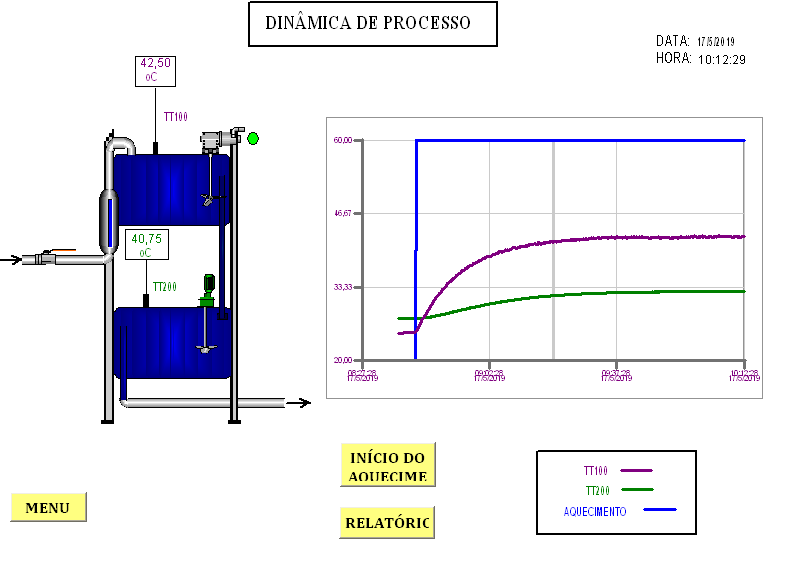
\includegraphics[scale=.8, trim={0 0 0 0}]{figuras/ladeq/dina/ft2}
		%\vspace{-20pt}
		\caption{Tanques abertos, em série, com agitação e sistema de aquecimento no primeiro tanque.}
		\label{aparato}
	\end{center}
\end{figure}

\section{Procedimento experimental}

Dois tanques em série possuem a mesma vazão de entrada e saída e estão com aproximadamente a mesma temperatura no início do processo ($ T1 = 24,82 \  ^{\circ}C \  e \ T2 =24,62 \ ^{\circ}C) $; Em determinado momento, aciona-se o aquecedor acoplado ao primeiro tanque, promovendo uma perturbação degrau no sistema que o induz a um comportamento transiente durante determinado tempo até que um novo estado estacionário seja obtido. Tal momento, de início do aquecimento, é registrado na figura 2 pela linha azul no gráfico. 

A perturbação é monitorada por dois sensores que, conectados a um computador, acompanham a variação da temperatura nos dois tanques. No iFix (software utilizado para acompanhamento do processo), as curvas TT100 (curva roxa) e TT200 (curva verde) representam as temperaturas dos tanques 1 e 2, respectivamente, ao longo do tempo. Pode-se observar que após certo período, o novo valor de temperatura foi estabilizado em $ 42,5 \ ^{\circ}C $ no tanque 1 e $ 40,75 \ ^{\circ}C  $no tanque dois. A ligeira diferença se deve ao fato do tanque 1 receber diretamente o aquecimento.


\begin{figure}[H]
	\begin{center}
		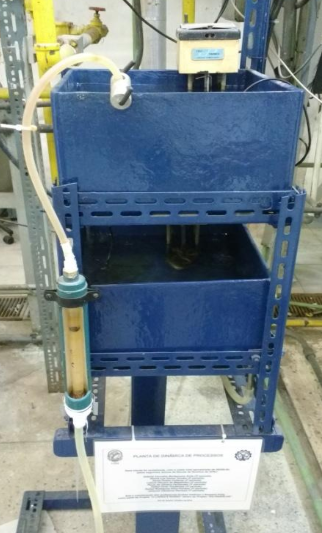
\includegraphics[scale=.8, trim={0 0 0 0}]{figuras/ladeq/dina/ft1}
		%\vspace{-20pt}
		\caption{Monitoramento da prática obtida através do software iFix.}
		\label{iFix}
	\end{center}
\end{figure}


\chapter{Cálculos}


Pela Tabela \ref{tab1} podemos observar quanto tempo levou, após acionarmos o aquecimento, para que cada tanque iniciasse seu aquecimento. Esse tempo entre o acionamento e o inicio dos efeitos na variável controlada foi estimado como o tempo morto do sistema. 

\begin{table}[H]
	\centering
	\begin{tabular}{|c|c|c|}
		\hline
		\textbf{t(s)}                 & \textbf{T2}                   & \textbf{T1}                   \\ \hline
		0.00                          & 24.88                         & 25.15                         \\ \hline
		...                           & ...                           & ...                           \\ \hline
		\cellcolor[HTML]{F8FF00}3.00  & 24.88                         & \cellcolor[HTML]{F8FF00}25.15 \\ \hline
		4.00                          & 24.82                         & 25.21                         \\ \hline
		...                           & ..                            & ..                            \\ \hline
		\cellcolor[HTML]{FCFF2F}50.00 & \cellcolor[HTML]{FCFF2F}24.88 & 26.19                         \\ \hline
		51.00                         & 24.95                         & 26.25                         \\ \hline
	\end{tabular}
\caption{Valores definidos como constantes de tempo morto para T1 e T2.}
\label{tab1}
\end{table}

Portanto o tempo morto para o tanque 1, ou seja, $ t_{01} $ é igual a 3 segundos. Já o tempo morto para o segundo sistema, $ t_{02} $ é igual a 50 segundos.

Foi determinada então a amplitude da perturbação. Durante o experimento foram coletados dados do aquecedor elétrico utilizando um multímetro, foi medida a corrente e a tensão do aquecedor. Com esses valores foi possível calcular a potência do aquecedor com base na Equação \ref{pot}:

\begin{equation}\label{pot}
\text{Potência}= \text{Tensão} \cdot \text{Corrente} = 125 V \cdot 9 A=1125 W
\end{equation}

\section{Cálculo das constantes para o Tanque 1}

Forma geral da função de transferência para um sistema de primeira ordem exemplificado pela Equação \ref{1ordem}.
\begin{equation}\label{1ordem}
G_{1}(s)=\frac{k_{1}}{\tau_{1} s+1} e^{-t_{01} s}
\end{equation}

Cálculo dos parâmetros da função de transferência

\begin{equation}\label{key}
k 1=\frac{T_{1}-T_{0}}{\text {Degrau}}=\frac{\Delta T}{\text {Degrau}}
\end{equation}

\begin{equation}\label{key}
T_{1}\left(\tau_{1}\right)=0,632 * P * k_{1}
\end{equation}

Primeira ordem em função do tempo:

\begin{equation}\label{key}
T_{1}(t)=A k_{1}\left(1-\exp \exp \left(-\frac{\left(t-t_{01}\right)}{\tau_{1}}\right)\right)
\end{equation}

Calculando com os valores obtidos durante o experimento

\begin{equation}\label{key}
k 1=\frac{42,50-25,15}{1125}=0,01543 \ \frac{^{\circ} C}{W}
\end{equation}

\begin{equation}\label{key}
\left[T_{1}\left(\tau_{1}\right)=0,632 \cdot P \cdot k_{1}=0,632 \cdot 1125 \cdot 0,01543=10,97073^{\circ} C\right.
\end{equation}


De posse dos valores obtidos no experimento, a temperatura do Tanque 1 estava em T1 = 25,15 +10,97 = 36,12073 em t = 749 segundos. Considerando o tempo morto, teremos 752 segundos.]

Chegamos então a seguinte função de transferência:


\begin{equation}\label{key}
G_{1}(s)=\frac{0,01543}{752 s+1} e^{-3 s}
\end{equation}


\begin{equation}\label{key}
T_{1}(t)=17,36\left(1-\exp \exp \left(-\frac{(t-3)}{749}\right)\right)
\end{equation}
 
Plotar o experimental juntamente do calculado:

\begin{figure}[H]
	\begin{center}
		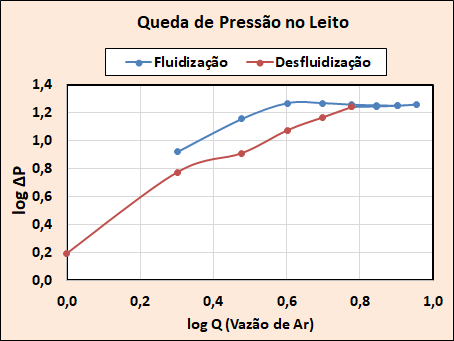
\includegraphics[scale=.5, trim={0 0 0 0}]{figuras/ladeq/dina/graph1}
		%\vspace{-20pt}
		\caption{Dados experimentais e dados obtidos da função de transferência em variável desvio.}
		\label{iFix}
	\end{center}
\end{figure}


\section{Cálculo das constantes para o Tanque 2}

Considerado um sistema de segunda ordem já que existiam dois sistemas de primeira ordem em série:

\begin{equation}\label{key}
G_{2}(s)=\frac{k_{2}}{\left(\tau_{21} s+1\right)\left(\tau_{22} s+1\right)} e^{-t_{02} s}
\end{equation}

Outra forma de se representar um sistema de segunda ordem é dado pela Equação \ref{2ordem}

\begin{equation}\label{2ordem}
G_{2}(s)=\frac{k_{2}}{\tau^{2} s^{2}+2 \xi \tau s+1} e^{-t_{02} s}
\end{equation}


Onde:

\begin{itemize}
	\item $ 2 \xi \tau=\tau_{21}+\tau_{22} $;
	\item $ \tau^{2}=\tau_{21} * \tau_{22} $.
\end{itemize}


Cálculo dos parâmetros da função de transferência:
\begin{equation}\label{key}
k 2=\frac{T_{2}-T_{0}}{D e g r a u}=\frac{\Delta T}{D e g r a u}
\end{equation}

O cálculo do ganho estático pela mesma Equação utilizada para o Tanque 1.

\begin{equation}\label{key}
k 2=\frac{40,81-24,88}{1125}=0.01416 \frac{^{\circ} C}{W}
\end{equation}

Quanto as constantes do comportamento dinâmico do tanque 2, foram determinadas da seguinte forma:

\begin{equation}\label{key}
T_{2}\left(\tau_{2}=0,73\right)=0,73 \cdot P \cdot k_{2}=0,73 \cdot 1125 \cdot 0.01416=11,9475 \ ^{\circ} C
\end{equation}

O tempo correspondente ao valor de temperatura $ T_2= 24,88 + 11,95 = 36,83 \ ^{\circ}C  $ foi de 1848 segundos. Descontando o tempo morto de 50 segundos teremos t = 1798 segundos. Com a metade deste tempo e somando o tempo morto, determinou-se a resposta correspondente do sistema,$ T_{2}\left(\frac{t_{3336}}{2}+t_{02}\right)=T_{s}=T(t=949 s)=31.38-24.88=6,50 \ ^{\circ} C . $Assim, resolveu-se o seguinte sistema:


\begin{equation}\label{key}
\left\{\begin{array}{c}{t_{73\%}=1,3\left(\tau_{21}+\tau_{22}\right)} \\ {\frac{T_{s}}{A k_{2}}=\frac{\tau_{22}}{\tau_{21}}}\end{array}\right. \rightarrow \left\{\begin{array}{c}{\tau_{21}=\frac{t_{73 \%}}{1,3\left(1+\frac{T_{s}}{P k_{2}}\right)}=1009,59 \mathrm{s}} \\ {\tau_{22}=\frac{T_{s}}{P k_{2}} \tau_{21}=411,95 \mathrm{s}}\end{array}\right.
\end{equation}

Portando:

\begin{itemize}
\item $ \tau=\sqrt{\tau_{21} \cdot \tau_{22}}=\sqrt{1009,59 \cdot 411,95}=644,90 $
\item $ \xi=\frac{\tau_{21}+\tau_{22}}{2 \cdot \tau}=\frac{1009,59+411,95}{2 \cdot 644,90}=1,10 $
\end{itemize}


Com base no valor obtido para a constante de amortecimento do sistema, $ \xi $, podemos classificá-lo como um sistema superamortecido sem oscilação. O que de fato foi observado na resposta da temperatura do Tanque 2.

\newpage

Assim, função de transferência obtida é dada por:

\begin{equation}\label{key}
G_{2}(s)=\frac{0,01421}{(1009,59+1)(411,95 s+1)} e^{-50 s}
\end{equation}

Ou: 

\begin{equation}\label{key}
G_{2}(s)=\frac{k_{2}}{640,99^{2} s^{2}+2 \cdot 1,1 \cdot 640,99 s+1} e^{-50 s}
\end{equation}

Em função do tempo, o sistema de segunda ordem pode ser descrito como:

\begin{equation}\label{key}
T_{2}(t)=P k_{2}\left(1-\frac{\left(-\frac{\left(t-t_{02}\right)}{\tau_{21}}\right)-\left(-\frac{\left(t-t_{02}\right)}{\tau_{22}}\right)}{\tau_{21}-\tau_{22}}\right)
\end{equation}


A função dependente do tempo é dada por:


\begin{equation}\label{key}
T_{2}(t)=15.93\left(1-\frac{1009,59 \exp \exp \left(-\frac{(t-50)}{1009,59}\right)-411,95 \exp \exp \left(-\frac{(t-50)}{411,95}\right)}{813.81}\right)
\end{equation}


\begin{figure}[H]
	\begin{center}
		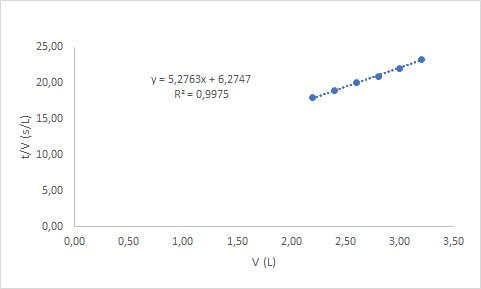
\includegraphics[scale=.5, trim={0 0 0 0}]{figuras/ladeq/dina/graph2}
		%\vspace{-20pt}
		\caption{Dados experimentais e dados obtidos da função de transferência em variável desvio.}
		\label{iFix}
	\end{center}
\end{figure}

Abaixo na Figura \ref{dois} é possível comparar o diferente comportamento dinâmico dos dois tanques. Em ambos os casos as curvas obtidas pela  metodologia empírica de determinação da função de transferência se correlacionaram muito fortemente com as previstas fenomenologicamente.




\begin{figure}[H]
	\begin{center}
		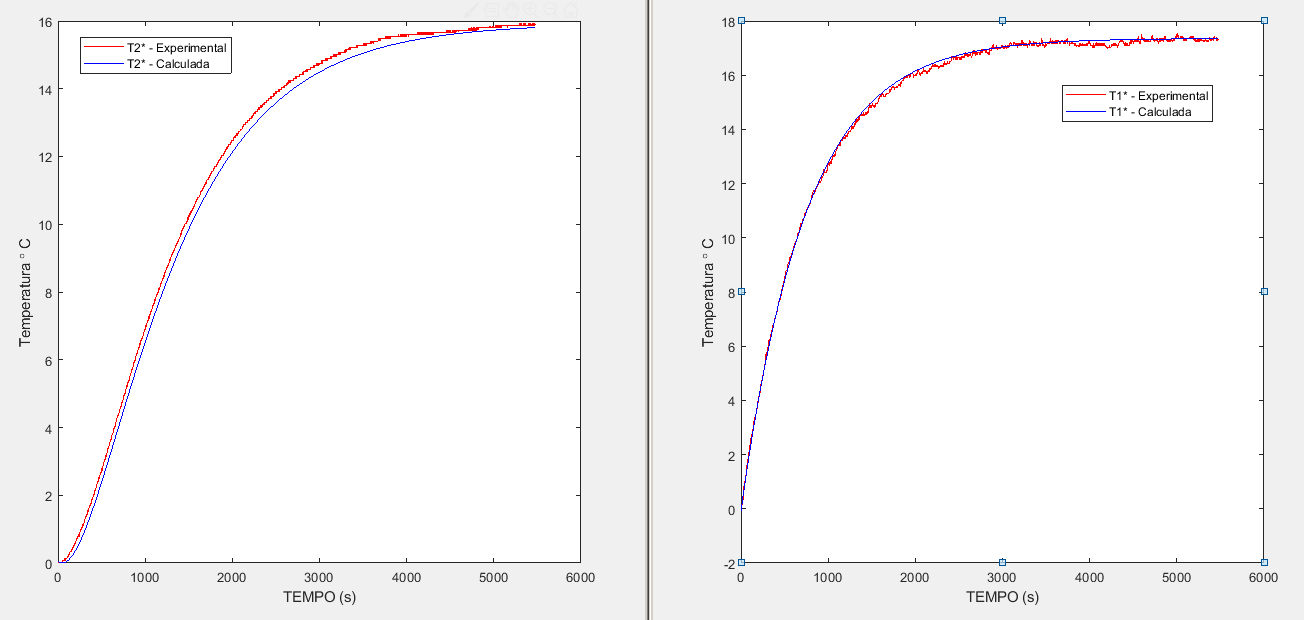
\includegraphics[scale=.5, trim={0 0 0 0}]{figuras/ladeq/dina/graph3}
		%\vspace{-20pt}
		\caption{Dados experimentais e dados obtidos para as temperatura dos Tanques 1 e 2.}
		\label{dois}
	\end{center}
\end{figure}


\chapter{ Conclusões}

De acordo com o que foi observado por meio dos dados obtidos na prática, pode-se concluir que as premissas adotadas de comportamento, de primeira ordem para o primeiro tanque, e de segunda ordem para o segundo tanque, num sistema de tanques agitados em série se mostrou válida. Ambas as curvas obtidas pelo modelo fenomenológico mostraram forte correlação com as os dados empíricos. No primeiro tanque o tempo morto foi pequeno, de apenas 3 segundos, indicando uma boa agitação, visto que a variação de temperatura foi prontamente detectada pelo termopar. Já no segundo tanque, houve um tempo morto maior, isto é de 50 segundos, uma vez que a variação de temperatura no segundo tanque dependia do aumento de temperatura do primeiro. 

O valor do coeficiente de amortecimento encontrado para o segundo tanque indica comportamento superamortecido (>1), o que pode ser corroborado pela curva que não apresentou caráter oscilatório como resposta à perturbação degrau.












